\documentclass[
  hyper,    
  lang=cn,
  class=book,
  mathSpec={envStyle=leftbar, alias},
  toc={redef}
]{zlatex}
\zcolorset{
  % link        = teal,
  definition  = blue
}
\usepackage[bottom]{footmisc}
% minted setup
\usepackage{minted}
\definecolor{bg}{rgb}{0.95,0.95,0.95}
\setminted{
  fontsize=\small,
  bgcolor=bg, 
  breaklines=true, 
  tabsize=2,
  breakanywhere=true,
  breakanywheresymbolpre=,
  breaksymbolleft=,
}
% print macro
\let\cmd\ztexverb
\newcommand{\Footnote}[1]{\stepcounter{footnote}\footnote[\thefootnote]{#1}}
\ztexframe{leftbar}[gray]
\newcommand{\zkey}[1]{\texttt{<#1>}}


\title{z\TeX{} Introduction}
\author{Eureka}
\date{\today}

\begin{document}
\maketitle
\frontmatter
\tableofcontents
\mainmatter
\part{Document}
\chapter{Introduction}
\section{简介}
\subsection{为何叫z\TeX{}?}
% 也不知道为什么这个系列名称要加以`z'的前缀,可能是因为个人爱好,或是因为觉得这个字母对自己而言有着一些别的意味。
% 最开始此系列中此包含一个基本的文档类,叫做 $\pi$\LaTeX{}, 但是后面自己想开发一个用于绘图的宏包,主要基于TiKZ.
% 用于常见平面图形的绘制以及外部程序的交互. 也许是看到了\cmd{tikz}库名称中的``z'',于是便以`z'为前缀,产生了
% z\LaTeX{}系列。


初看本系列的命名 z\TeX{} 可能会给使用者以某些滑稽的感觉. 为何要加以前缀以字母 ``z'', 也许应是许多用户想知道的问题.
下面就是可能的几点原因:

(1) 看到 \LaTeX3 开发团队挺喜欢用 ``x'' 来作为他们开发的一系列宏包的,比如 xparse, xcoffins, xfp等。我自然不能直接抄袭,
所以就用冠以字母 ``z''. 一方面 ``x→y→z'',有了``x'', 才有 ``z''(z\TeX{} 全程基于\LaTeX3 进行开发,
可以说,没有\LaTeX3, 就没有今天的z\TeX{}). 所以 ``y'' 去哪里了? 当你加入 z\TeX{} 的开发后, 就有 ``y'' 了.

(2) 如果你旋转一下字母 `z` 其实就得到 ``阿列夫 - $\aleph$''了,其实就是希望 z\TeX{} 系列能够有一些能够拓展的可能
(当初在设计这个系列之初便一直坚持模版的可拓展性)。所以用户如果想要深入使用本系列,那么可以在目前提供的基础接口(如缓存,
外部交互,内置utils)上可以拓展自己喜欢的功能, 一起把 Z\TeX{}, 打造成 ``$\aleph$ TeX''. 这也是我在本系列设计之初就有的
一个比较美好的,宏大的,不切实际的愿望,尽管可能性很低,但如果它实现了呢? 

(3) 最后可能还是因自己有想要打造一个类似 C\TeX{} 宏集的目标:尽管我知道以我目前我的水平还是远远不够的,所以现在我把这个``Z\TeX{}''就交给社区了,
希望在将来的某一天,人们在谈到 ``C\TeX'' 时也会想到有一个和它类似的宏集 -- ``Z\TeX{}''.


\subsection{为何用 z\TeX{}?}
为什么要用我的工具/模板?现在ztikz的几个外部交互模块其实是处于一种比较尴尬的境地的,我如果会用这些程序,
那么我单独使用这些程序可以调整图片的所有细节,然后输出图片,最后在 \LaTeX{} 中插入。如果我不会使用这些程序,
那么在正常使用这些模块前,我还需要自行安装对应的程序,那我为何不自己花时间去学学这个应用/程序,从而像第一种方法
那样直接在外部把图片(生成)处理好,然后再插入呢?

所以现在又回到这个问题了:我会用 \LaTeX{} 自己写模板,那我为什么还要用你的模版呢?我如果不会用 \LaTeX{} 写模板,
花费同样多的时间去了解你这个模板的使用细节,为何我不把这时间用在我自己去学习 \LaTeX{}, 这样反而能做出更加满足自己需求的模板 ? 
最终还可以得出:我为什么一定要用 \LaTeX{} 呢? 难道用成熟的软件,如 Word, Indesign 甚至是手写就不能写一篇工整规范的论文/笔记 ? 
所以为什么 Knuth 老爷子要花费十年的时间去开发 \TeX{} 呢? 

上述的一系列推论正确吗?稍微仔细去想,你会发现上面的推导确实不都是正确的。前一个条件并不一定是充分的,或者说我们使用了一个
假命题(关系)去得到了另一个命题(关系)。根据基础的逻辑知识:定义汇集 $\text R \vee \text S$ 为两关系 R, S 的逻辑析取,定义
汇集 $\lnot \text R$ 为关系 R 的逻辑否定。从而我们就可以定义我们所谓的 ``逻辑蕴含'' 关系 $\lrr{}$, 即记号 $\text R\lrr{} \text S$ 
其实是如下的关系汇集:
\[
  \text S \vee (\lnot \text R)
\]

在我们定义了关系 ``真'' 后,如果关系 $\text R\lrr{}\text S$ 是真的, 那么:
\begin{itemize}
  \item 如果关系 R 时真的,那么关系 S 必然是真的,也就是我们得到了一个 ``真'' 的结论
  \item 但是如果 R, S 同时为假,那么关系 $\text R\lrr{}\text S$ 也是真的.但是此时我们的结论并不是``真的'',也就是结论并不成立.
\end{itemize}

\begin{remark}
其实有 $\lnot, \vee$ 这两个基础的符号就已经能表示出很多的关系了, 比如逻辑合取记号: $\text R\wedge \text S$ 其实就是:
$ \lnot [(\lnot \text R)\vee (\lnot \text S)]$. 在规定逻辑公理后其实就可以用来说明我们常用的 ``三段论,双重否定''等
常见逻辑推理了. 比如我们常用的逆否命题就是说: 关系 $(\text R\lrr{}\text S) \lrr{} ((\lnot\text S)\lrr{}(\lnot\text R))$
是真的.
\end{remark}

可以认为我们用一个假命题导出了另一个假命题, 下面以此来说明z\TeX{}值得你用,我要如何说服你去使用我的模板呢? 当然就是
让 ``R\; \lrr{} S''中的命题 ``R'' 为假就好了。比如,我可以让我的模板上手难度相较于默认的 \LaTeX{} 低一点,那么要达到
同样的效果,你所花费的时间就少一点。所以上述``花费同样时间''这一个命题就为假, 所以``z\TeX{}值得你用'' 这一命题论证完毕。
你也许可以找到其他的论据来反驳我,但是至少我找到了一个论据来说服你,也找到了我开发这个系列的初心.

\subsection{项目地址}
目前本项目已经在GitHub, Gitlab, Gitee上开源,地址如下:
\begin{itemize}
    \item GitHub: \href{https://github.com/zongpingding/ZLaTeX_ZTikZ}{https://github.com/zongpingding/ZLaTeX\_ZTikZ}
    \item Gitlab: \href{https://gitlab.com/zongpingding/ZLaTeX_ZTikZ}{https://gitlab.com/zongpingding/ZLaTeX\_ZTikZ}
    \item Gitee:  \href{https://gitee.com/zongpingding/ZLaTeX_ZTikZ}{https://gitee.com/zongpingding/ZLaTeX\_ZTikZ}
\end{itemize}

项目中包含z\LaTeX{}文档类源码\cmd{zlatex.cls},zTikZ宏包源码\cmd{ztikz.sty},以及二者的说明文档. 后续在开发过程中,
可能会保证Github的同步更新,至于Gitlab与Gitee则不一定会同步本系列的最新版.

z\LaTeX{}系列源代码完全开放,欢迎各位对源代码的修改以及二次分发. 如果想要和我一同改进此模板,请在
Github提Issue或者是PR. 不要在Gitee或者是Gitlab上提问,本人只维护Github上的仓库,尽管有时可能会为了
国内用户下载方便,把Github上的仓库同步到这两处. 

作为一个完全免费(为爱发电)的项目,我不对任何本模板的使用者负责,如果使用者在使用后遇到任何的严重后果,我不负
任何责任. 我很乐意给大家解决问题,但是在提问前请先了解\LaTeX{}提问规范,一起营造一个愉快的讨论氛围. 

想要体验本模板请到Github仓库:\href{https://github.com/zongpingding/ZLaTeX_ZTikZ/releases}{Release界面}下载 
对应的最新模板. 由于本模板现在正处于早期开发阶段,所以很多的接口并不稳定,不保证模板的向后兼容性,请各位见谅.

\subsection{基本组成}
本系列目前包含以下的三个组成部分,一个文档类,一个beamer宏包以及一个绘图库:
\begin{itemize}
    \item z\LaTeX{} 文档类
    \item zTikZ 宏包
    \item zSlide 宏包
\end{itemize}

其中前者主要用于指定排版文档的基本属性,zTikZ宏包主要用于绘图\Footnote{众所周知的,在\LaTeX{}中绘图是一件十分痛苦的事情,
于是乎你会看到很多书籍或笔记中的图形都是手绘或者是截图,并非矢量图},最后一个 zslide bemaer 宏包是自己设计的一套 beamer 主题。
尽管 z\LaTeX{} 本身也可以在加上 \cmd{layout/slide} 选项后称为一个演示文档,但是在严肃的场景下,还是推荐使用 beamer 文档类.

其实从这个介绍文档就可以看出,本模板是十分的朴素的,没有十分华丽的色彩和精美的页面布局,但是在折腾了许久的\LaTeX{}之后,现在这个
模板才是最对我胃口的;至于,是否适合你,那就不得而知了。你可以去使用更加精美的模板,比如 \href{https://github.com/ElegantLaTeX}{Elegant\LaTeX{}}, 
\href{https://github.com/BeautyLaTeX/Beautybook}{Beauty\LaTeX{}} 等优秀的模板. 

\begin{remark}
后续可能还会开发一个 zTool 宏包,作为 z\LaTeX{} 系列的补充.
\end{remark}

\subsection{使用手册}
本文档中的\cref{模板设计}一般的使用者可以跳过,这一部分主要是我自己对本模板的设计思路和关于写\LaTeX{}的个人感受,
对于使用模板和宏包而言,没有任何的帮助.如果要了解\cmd{zlatex.cls}文档类的使用,请直接跳转到``z\LaTeX{}文档类教程''
文档:zlatex\_manual.pdf. 如果要了解\cmd{ztikz.sty}宏包的使用,请跳转到zTikZ宏包教程文档:ztikz\_manual.pdf.
目前 zslie 还没有对应的文档说明,仅有一个示例: zslide\_manual.pdf.



\chapter{模板设计}\label{模板设计}
\section{设计历程}
本模板的设计经历了相当长的一个周期,从最开始的初始\LaTeX{},我把自己常用的宏扔到了一个\cmd{.sty}文件中,以为这就是
一个宏包了;之后了解到了 \href{https://github.com/ElegantLaTeX}{Elegant\LaTeX{}} 系列模板,也使用这个系列中的 eleganbook 
文档类写了一点自己的笔记,但是用了一段时间之后总归是不满意,很多地方都想要自己定制,不喜欢模板默认的样式;奈何自己当时的水平不够,
打开模板,映入眼帘的源码对于我来说和一堆乱码无异。后面自己看了一些文章后,慢慢积累,渐渐对\LaTeX{}熟悉了一些,这才开始着手设计模板。

第一版的 z\LaTeX{} 可以说完全是照抄的 elegantbook 文档类,但是自己又加了一些东西,进行了一些简单的修改,比如字体,颜色等等。
但是写到后面,发现这个模板变得十分的混乱了, 代码的结构不好控制了\Footnote{其实最开始这个zTikZ宏包和z\LaTeX{}是一体的,当时代码极其混乱}.
其中的选项配置接口写起来是极其痛苦的, 以其中的模板语言切换为例,下面就是当初写的那个\cmd{\ifdefstring}对应的代码片段:

\begin{minted}{latex}
\DeclareVoidOption{cn}{\kvs{lang=cn}}
\DeclareVoidOption{en}{\kvs{lang=en}}
\DeclareStringOption[cn]{lang}
\end{minted}

感觉很麻烦,有没有? 加之, 当时基本文档类为\cmd{article},很多\cmd{book}文档类的内部计数器和章节命令都没有,需要自己去声明;
但是结果往往是:自己设计的命令和别的宏包不兼容. 其中的\cmd{hyperref}宏包折腾了我许久,初代模板中由于自己定义的计数器不正确,
所以跳转功能不正常. 比如在使用\cmd{\label}命令时,激活的章节元素(跳转位置)不对。当初的目录也有着同样的跳转问题.

另一方面,初代 z\LaTeX{} 文档类全采用 \LaTeX{}2$\varepsilon$ 进行构建,很多涉及到宏展开的地方写的很繁琐不直观。且由于当时水平所限,
模板中大部分的实现方案都是抄袭的 \TeX-StackExchange 上的回答。这就导致,很多时候这个模板都是处于一种能跑的状态,但是我并不知道具体命令的
作用. 

\subsection{z\LaTeX{}}
后来自己把zTiKZ从中 z\LaTeX{} 文档类中剥离出来,同时使用 \LaTeX{}3 对原始文档类和 zTikZ 进行重构.其中z\LaTeX{}文档类默认加载\cmd{book}
文档类,也可以加载其余的文档类. 之后几乎所有命令都先去了解原理,知道它们的具体作用,对其他的宏包的影响, 然后自己构建。于是 z\TeX{} 系列就诞生了.
果然,在使用\LaTeX3对原始项目进行重构之后,整个项目的代码清爽了许多, 整个项目的开发效率也提高了许多. 比如下面 z\LaTeX{} 文档类的加载选项声明:

\begin{minted}{latex}
\zlatex_define_option:n {
    % language
    lang                  .str_gset:N   =  \g__zlatex_lang_str,
    lang                  .initial:n    =  { en },
    % page layout
    layout                .str_gset:N   =  \g__zlatex_layout_str,
    layout                .initial:n    =  { twoside },
    % margin option
    margin                .bool_gset:N  =  \g__zlatex_margin_bool,
    margin                .initial:n    =  { true },
}
\ProcessKeysOptions {zlatex / option}
\end{minted}

看着是否清爽了许多? 但是后面发现这样还是不够的方便,问题在于:如果你需要加载的子文档类的选项比较多时,你需要声明许多这样的
key-value,当整个文档类的 key-value 声明过多时,模板便会变得难以维护。所以这是引入了 l3keys2e 中\textbf{元键}(\cmd{.meta:nn})。
作用便是: 用于将所有的 key-value 根据模块进行层级划分, 在指定时也按照模块进行指定. 下面就是目前的 z\LaTeX{} 文档类的键值对接口:

\begin{minted}{latex}
\zlatex_define_option:n {
    % zlatex language
    lang            .str_gset:N   =  \g__zlatex_lang_str,
    lang            .initial:n    =  { en },
    % class and options
    class           .str_gset:N   = \g__zlatex_subclass_type_str,
    class           .initial:n    = { book },
    classOption     .clist_gset:N = \g__zlatex_subclass_option_clist,
    classOption     .initial:n    = { oneside, 10pt },
    % zlatex options meta key 
    layout          .meta:nn      = {zlatex / layout}{#1},
    mathSpec        .meta:nn      = {zlatex / mathSpec}{#1},
    font            .meta:nn      = {zlatex / font}{#1},
    bib             .meta:nn      = {zlatex / bib}{#1},
    ...
}
\end{minted}

同时声明的 \texttt{<classOption>} 可以轻松简单的处理子文档类的加载选项问题.

\subsection{zTikZ}
对于宏包 ztikz.sty,其开发也经历了也很长的时间. zTikZ 也从最开始的一个大宏包变成了一个个的小的子模块:
cache, python, gnuplot, wolfram 和 zdraw. 这些模块通过如下命令:

\begin{minted}{latex}
\ProvidesExplFile{ztikzmodule.cache.tex}{2024/06/15}{1.0.0}{cache~module~for~ztikz}
\end{minted}

进行声明, 然后在主宏包 ztikz.sty 中声明如下命令来进行模块的调用:
\begin{minted}{latex}
\cs_new_nopar:Npn \g__ztikz_load_module:n #1 {
  \clist_map_inline:nn {#1} {
    \file_if_exist_input:nF {modules/ztikzmodule.##1.tex} {}
  }
}
\NewDocumentCommand\ztikzLoadModule{m}{
  \g__ztikz_load_module:n {#1}
}
\end{minted}

在处理好上述的模块划分以及接口声明后,对应的宏包使用者便只需通过:
\begin{minted}{latex}
\ztikzLoadModule{cache, python}
\end{minted}

进行相应的模块的单独调用.而且,在划分好模块后,不但可以方便宏包的使用者,更让我可以对不同的模块进行单独开发,我认
为这大大的提高了开发效率.

\section{设计参考}
本系列从诞生之初便由我一个人一直开发,在开发过程中参考了诸多优秀文档类/模板,参考最多的{C\TeX{}art}文档类,几乎是
本项目的大部分代码思路来源。此文档类完全采用\LaTeX3语法写成,本文档类中的\textbf{选项配置}模块主要参见\TeX-StackExchange上
的讨论,采用了\LaTeX3的l3keys2e模块;这样的好处有:选项配置简洁,符合用户习惯,模板维护方便.


\section{设计原则}
其实这个标题有一点太大了,什么是设计原则,我也不知道,但是我想让我的模板看着舒服。怎么才能让自己的模板看着舒服呢 ?
我也不知道,但是至少,应该,大概和页边距,字体大小,字体样式等有关吧。并且这三者之间也不一定时是独立的,
应该是相互影响的. 比如你的页边距变大,压缩了你的版心大小,那此时正文字体一定得做相应改变. 

现在的具体问题为:一行多少个字合适呢? 去查了一下\TeX.SE, 针对于英文,一行的字母个数在 65-90 是比较合适的,并且字体尺寸
一般为\cmd{10pt,11pt,12pt};页边距到底设置多少呢? 自己去比对了如 Elegantbook 和其它模板的页边距也发现了一些东西. 
当时测量各种距离很不方便,就差用尺子量了,但是后来我发现了一个宏包 fgruler. 它可以在生成的 PDF 中直接打印输出页面布局尺寸,
使用方法也很简单:

\begin{minted}{latex}
\usepackage[hshift=0mm,vshift=0mm]{fgruler}
\end{minted}

当你在导言区引入之后,便可以在你的每一个页面上看到如\cref{fig:fgruler-example}的输出, 这样就不用你用尺子量了.

\begin{figure}[!htb]
    \centering
    
\includegraphics[width=.45\linewidth]{fgruler_1.pdf}
    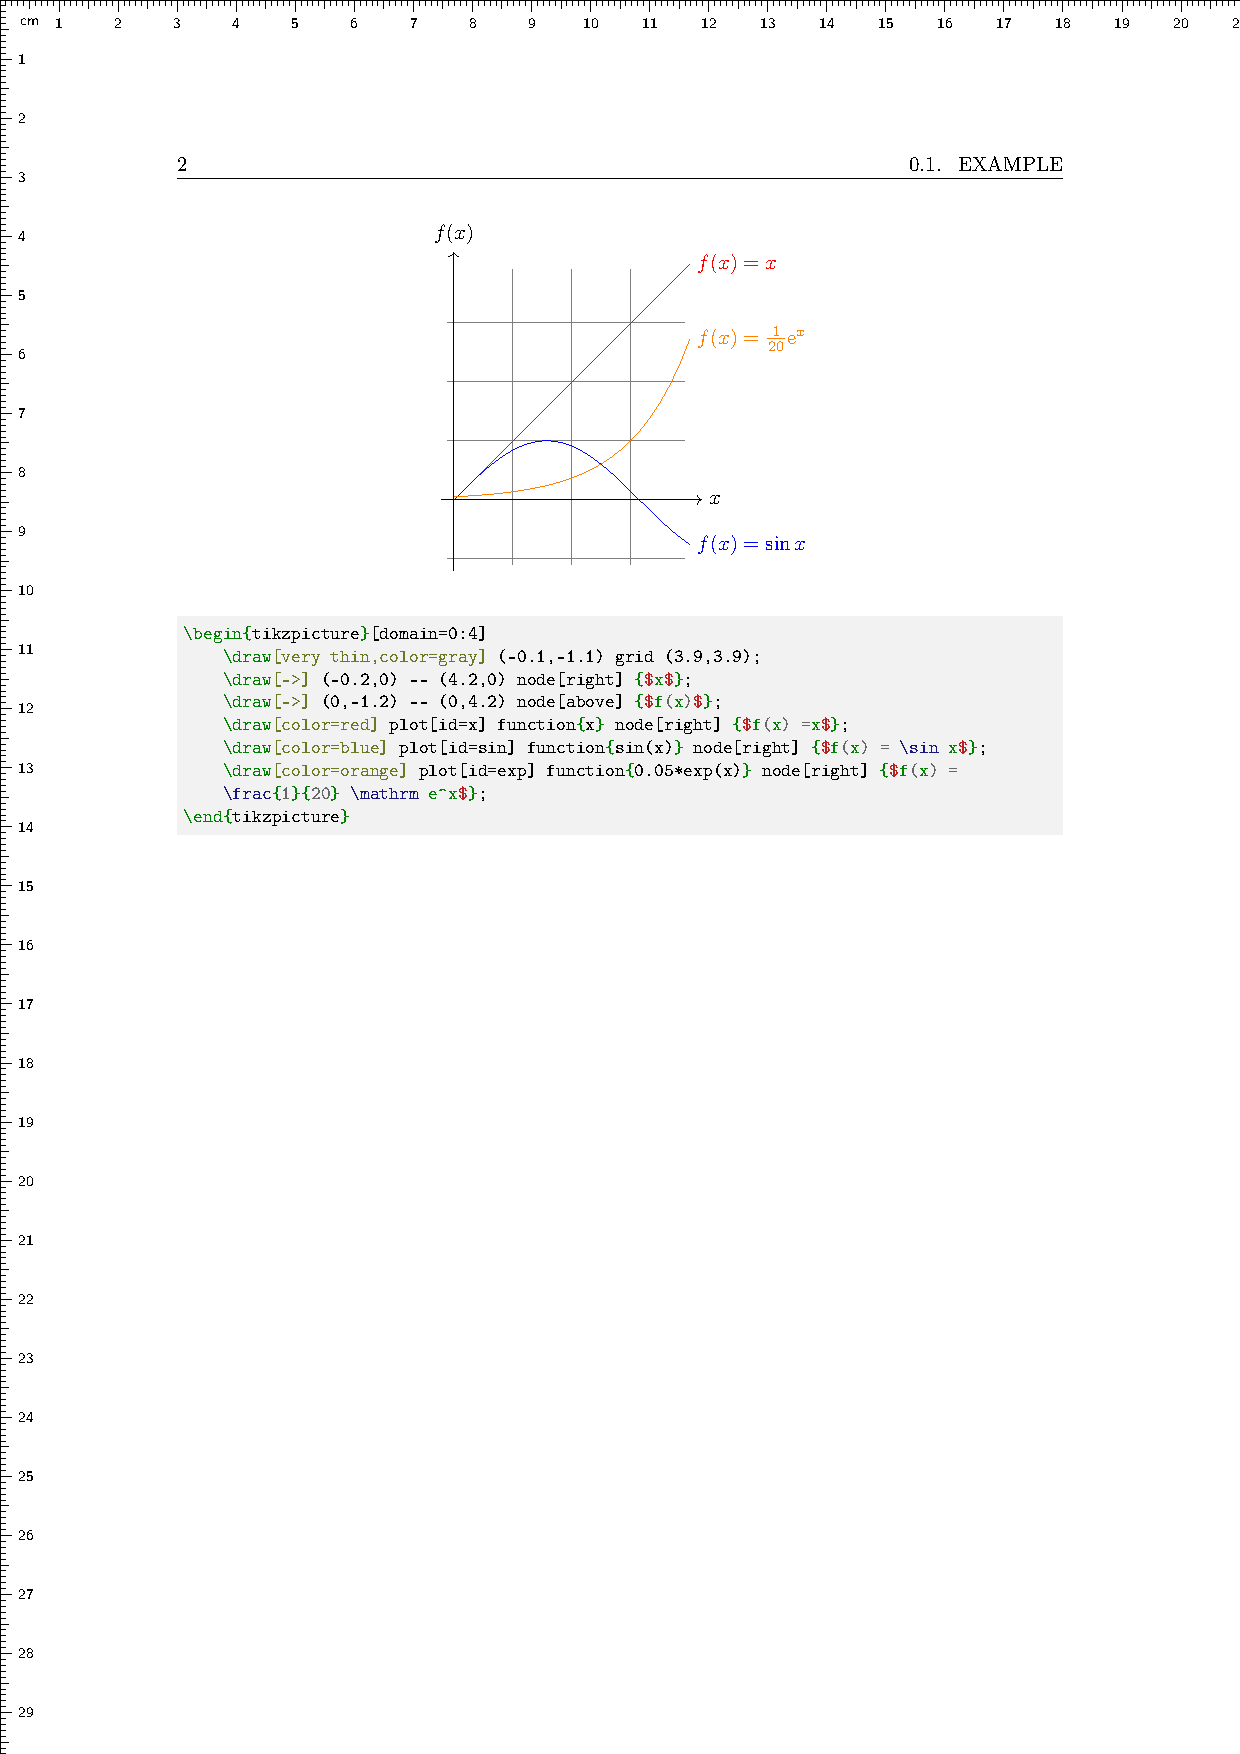
\includegraphics[width=.45\linewidth]{fgruler_2.pdf}
    \caption{页面布局示意图}
    \label{fig:fgruler-example}
\end{figure}

在设计本模板的时,我也一直在纠结字体的问题,我应该把字体打包进入模板吗? 或者是我应该在模板中给用户进行默认的字体设置吗?
在这个系列的上一版中我就去找了一些免费的中文字体和西文字体,直接放在模板的文件夹下,但是这样产生的问题就很多了:

\begin{itemize}
    \item 用户需要这个字体吗, 增加的字体会变成这个模板的负担吗 ?
    \item 这个字体真的免费吗 ?
    \item 中文字体的字形往往是不全的,怎么解决 ? 
\end{itemize}

于是最终的办法就是,我的模板不负责字体的设置,不添加任何和字体相关的配置,所有的字体由用户指定. 但是,毕竟是作为了一个模板,
所以我还是提供了部分有关数学字体的配置,可以供用户选用,如果用户确实需要这个字体。

在设计这个模板时,行距等各种元素的设置也难倒了我一段时间。所以设计一个模板,你考虑的东西是很多的。但是自己也得到了一个规律:如果某些配置你不会,
那么就让它们保持默认. \textcolor{red}{Be simple, Be fool}.

Anyway, 尽管有着种种的困难,z\TeX{} 还是没有烂尾, 最终出现在了大家的面前. 

\section{无题}
时至今日,再次回头来看我的这个模板,我反而有了一些其他的感受. 一个模板到底需要给用户定制什么东西 ? 到底需要给用户
多大的自由空间(配置选项)? 如果你的配置选项过多,像 \href{https://www.ctan.org/pkg/koma-script}{koma-script}, 
\href{https://ctan.org/pkg/memoir}{Memoir} 那样, 模板作者给用户处理了很多的细节,提供了种类繁多的接口. 或者像部分简单
的模板仅提供几个必要的设置和命令; 而且,如果一个模板的说明文档都达到了上百页,那么我作为一个用户为什么不自己学习做模板,写一个
适合自己的模板,反而要话这部分时间来学习使用你的模板? 如果模板的配置选项过少,那么用户又会觉得这个模板不够灵活. 所以,
到底什么样的一个模板设计才能够称得上是:\textcolor{red}{简单,灵活,易用}? 遗憾的是,现在我也没有办法回答这个问题,所以这个问题作为习题,
留给使用者回答了 ...

z\LaTeX{} 系列写到今天,它已经不再是一个简单的``文档类+绘图库+slide''了,所以这个系列可能并不适合新手. 同时我也意识到,很多时候
其实我们并没有必要非得写一个模板出来,你需要什么样的功能,你就去找什么样的宏包,然后调用它,根据它提供的命令实现自己的需求.这样才会更加
符合自己的需求,而且你也不用去考虑太多的兼容性问题, 更没有必要去花费那个你在使用别人模板时阅读模板细节的时间. 似乎,有了基础文档类 
article, book 以及各种功能性宏包之后,\LaTeX{}就已经足够好了, 并不需要我们这些闲来无事的人写来写所谓的模板 ? 反而我是觉得:应该把更多的时间
花在基础宏包的开发上,就像 pgf, l3draw 等宏包那样:我只提供基础的几组底层绘制命令,至于上层的封装,那就交给用户去实现吧. \texttt{>\_<}


\chapter{敬告}
\section{兼容性}
目前本系列已经实现Windows和Linux下的兼容; 但是MacOS下:目前仅支持z\LaTeX{}文档类.
zTikZ还未进行适配(参见下文了解具体原因),所以不保证本系列中的zTikZ文档类可以在MacOS下正常运行.
具体的兼容情况请参见后续的兼容性章节.

\section{说明文档}
\subsection{记号说明}
本系列宏集的所有手册均遵守如下规范:
\begin{itemize}
  \item 命令或者部分的专业术语采用打字机字体进行给出
  \item 所有的命令均使用格式 \cmd{\cmd}进行标注
  \item 所有的键值对均使用\zkey{key}进行标注,或者采用打字机字体强调.
\end{itemize}



\subsection{手册编译}
本系列的所有文档类或者是宏包的使用手册对应的\TeX{}源文件均可以在Github仓库下载,但是如果你想要编译此文档,
那么还请参看如下的编译环境配置:

\begin{itemize}
    \item 首先清除之前的编译文件,比如\cmd{.aux}, \cmd{.log}, \cmd{.toc}等文件以及
        \cmd{ztikz_output/}文件夹。
    \item 使用\cmd{xelatex}编译此文档,编译两次。(如果第一次编译报错\cmd{missing \begin{document}...})
        那么请注释掉主文件\cmd{zlatex_ztikz_doc.tex}中和\cmd{indextool}相关的两行语句:\cmd{\makeindex[]{}},
        \cmd{\printindex[]{}},然后再次编译. 如果你想要生成索引,请取消注释上一步中的两行语句,
        然后再次编译.
    \item Want Build From Scratch? 那么需要本地环境中有配置好的: WolframScript, gnuplot, Python, Sed.
\end{itemize}

\subsection{复制样例}
本文档中给出了相当部分的样例及其对应的代码,在书写本文当时为了读者的阅读体验,对代码抄录环境中的部分符号进行了
重写。比如你会在代码中看到换行符为:$\hookrightarrow$,那么在复制此环境代码时,请删掉此符号。亦或者是源代码中有行号,
那么在复制后,请删掉多余的行号. 亦或者是,后续的 Implement 节中部分的代码换行,请把不必要的换行符删掉再进行编译.

\subsection{键值指定}
本系列中的大部分命令均采用键值对的形式进行调用, 使用 \zkey{key}的形式给出. 所以如果一个命令的可用键太多,那么此时我并不
一定会在正文中全部说明其可用键。我会在对应的命令下方插入一个源代码抄录,用于说明此命令对应的声明原型,其中就包含了此命令可用的键值以及不同键
的默认值. 下面以一个具体命令 \cmd{\Polygon} 来说明怎么使用键值对接口:

\begin{minted}{latex}
% key-value setup
\keys_define:nn { ztikz / polygon }{
    radius       .fp_set:N  = \l__polygon_radius_fp,
    radius       .initial:n = { 1 },
    edgeColor    .tl_set:N  = \l__polygon_edge_color_tl,
    edgeColor    .initial:n = { black },
    fillColor    .tl_set:N  = \l__polygon_fill_color_tl,
    fillColor    .initial:n = { white },
    fillOpacity  .fp_set:N  = \l__polygon_fill_opacity_fp,
    fillOpacity  .initial:n = { 0 },
    rotate       .fp_set:N  = \l__polygon_rotate_angle,
    rotate       .initial:n = { 0 },
    shift        .tl_set:N  = \l__polygon_shift_tl,
    shift        .initial:n = { (0,0) },
    marker       .tl_set:N  = \l__polygon_marker_option_tl,
    marker       .initial:n = { },
}
% command
\NewDocumentCommand\Polygon{ O{}m }{
    \group_begin:
    \keys_set:nn { ztikz / polygon } { #1 }
    ... 
}
\end{minted}

上述的\cmd{\Polygon}命令即表示:此命令的第一个参数为一个可选参数(\cmd{O}类型),对应的选项指定方式为键值对.
可用的键有:\zkey{radius}, \zkey{edgeColor}, \zkey{fillColor}, \zkey{fillOpacity}, \zkey{rotate}, 
\zkey{shift}, \zkey{marker}等. 其中键\zkey{radius}可以接受一个浮点数(\cmd{\fp_set:N}), 默认值为
1(\cmd{.initial:n = { 1 }}); 再比如, 键\zkey{edgeColor}表示可以接受一个 tokenlist(\cmd{\tl_set:N}), 默认值为
黑色(\cmd{.initial:n = { black }}). 其余类似的键的选项指定方式类似,这里不再说明.


\end{document}